\begin{surferPage}[Sextic (30 חודים)]{משטח ממעלה שש של בארת' עם 30 חודים}
    לאחר שוולף בארת'
    \textenglish{ (Wolf Barth)} יצר את המשטח מהמעלה השישית עם המספר המרבי האפשרי
    של נקודות סינגולריות, $65$ (ראו גם משטח נוסף בגלריה זו)
    ושניים מהדוקטורנטים שהנחה יצרו גם הם משטחים ממעלה גבוהה יותר ששברו גם הם שיאי עולם,
    הוא החל לחקור את השאלה מהו המספר המרבי
    של חודים על משטחים ממעלה נתונה.

   בניית המשטח של בארת' בעל $65$ נקודות הסינגולריות מטיפוס
    $A_1^{+-}$ (חרוטים כפולים), ניתנת להתאמה לחודים; בדרך זו מתקבלים $30$ חודים
    : 
    \[P_6 - \alpha \cdot K^3=0,\]
  כאשר $P_6$ הם אותם מישורי סימטריה של האיקוזהדרון (עֶשרימוֹן) כמו עבור
    משטח בארת' האחר, וכאשר $K$ הוא
    שוב המשוואה של ספרת יחידה:
    \vspace*{-0.4em}
    \begin{center}
      \begin{tabular}{c@{\ }c@{\ }c@{\ }c}
        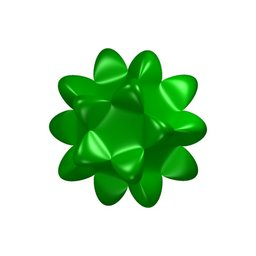
\includegraphics[height=1.2cm]{./../../common/images/barthsextic_30A2}
        &
        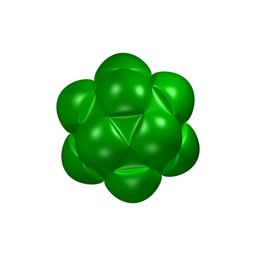
\includegraphics[height=1.2cm]{./../../common/images/barthsextic_30A2_3}
        &
        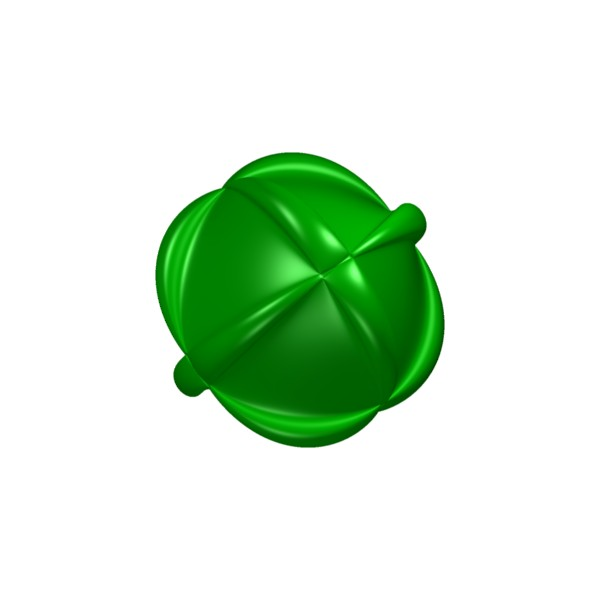
\includegraphics[height=1.2cm]{./../../common/images/barthsextic_30A2_5}
        &
        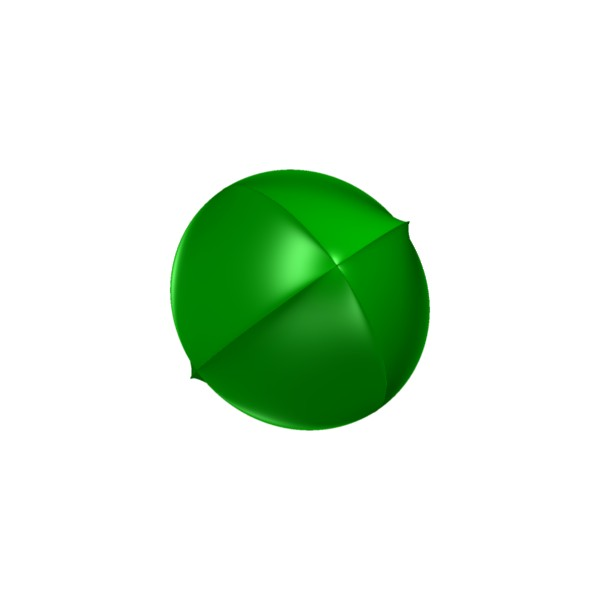
\includegraphics[height=1.2cm]{./../../common/images/barthsextic_30A2_6}
      \end{tabular}
    \end{center}    
    \vspace*{-0.3em}
     זהו השיא העולמי העדכני של המספר המרבי של חודים ממשיים
    במשטחים מהמעלה השישית. עבור חודים מרוכבים השיא עומד על $36$.
\end{surferPage}
